\documentclass[a4paper]{article}

\usepackage[english]{babel}
\usepackage[utf8]{inputenc}
\usepackage{amsmath}
\usepackage{graphicx}
\usepackage[colorinlistoftodos]{todonotes}
\usepackage{float}
\usepackage{caption}
\usepackage[font={scriptsize}]{caption}

\title{Battery Risk Prediction Challenge}

\author{Topcoder Handle: aukintux}

\date{\today}

\begin{document}
\maketitle

\begin{abstract}
The following document describes the various learning algorithms fitted to the dataset and the results obtained in the quest of optimizing the score metric. The various tasks were performed in a 8GB machine on Jupyter Notebooks.
\end{abstract}

\section{Score Metric}
\label{sec:score_metric}

Let us analyze the score metric for this challenge. The final score $F_s$ is defined as follows:

\begin{equation}
F_s = F_1 + 1 - \mathit{MRAE_c}
\label{eq:final_score}
\end{equation}

Where $\mathit{MRAE_c}$ stands for custom mean relative absolute error and is defined as follows:

\begin{equation}
\mathit{MRAE_c} = \frac{1}{N} \sum_{i}^{N} min\left(1, \left|\frac{P-G}{G}\right|\right) : G > 0
\label{eq:custom_mrae}
\end{equation}

This previous formula sums over all values whose ground truth value $G$ is greater than zero. Let us see that if the predicted value $P$ is $-1$, then, the component inside the sum will be $1$ since $G$ is greater than zero. 

This takes into account the requirement that: ``\textit{If P is -1, the relative absolute error is defined as 1}''.

\vspace{5mm}

The metric is then composed of two parts: $0 < F_1 < 1$ and $0 < \mathit{MRAE_c} < 1$. It is important to note that since $\mathit{MRAE_c}$ only sums through the samples whose ground truth label is strictly positive and in addition each component inside the sum is bounded from above by 1. Then, it is never a good idea for the algorithm to predict $P=-1$ since the results will hit the upper bound instantaneously.

\clearpage

\section{Algorithm Selection}
\label{sec:algo_selection}

In both cases the algorithms were fitted on the processed data and a 5-fold \textit{GridSearchCV} was used in order to find the \textit{best\_params\_}.

\subsection{$F_1$ Optimization}
In order to optimize the $F_1$ score where $\mathit{risk}=0$ is considered to be the positive class and $\mathit{risk} != 0$ is considered to be the negative class different classification algorithms were applied:

\begin{enumerate}
\item SVC
\item SVC with PCA
\item RandomForestClassifier 
\item RandomForestClassifier with PCA
\item DecisionTreeClassifier
\item DecisionTreeClassifier with PCA
\end{enumerate}

The best performing one was found to be the DecisionTreeClassifier. Even tough PCA can reduce the number of features to 50 with a cummulative variance of $99.37\%$ the algorithm without PCA is not computationally expensive. It takes less than 5 minutes to train and gives a light improvement.

\subsection{$\mathit{MRAE_c}$ Optimization}
In this case only the samples where $\mathit{risk} > 0$ where used in order to train the model. A few regression algorithms were fitted to the data:

\begin{enumerate}
\item ElasticNet
\item ElasticNet with PCA
\item SVR
\item SVR with PCA
\item RandomForestRegressor 
\item RandomForestRegressor with PCA
\item DecisionTreeRegressor 
\item DecisionTreeRegressor with PCA
\end{enumerate}

The algorithm that best performed was the DecisionTreeRegressor.

\section{Results}
\subsection{$F_1$ Score}
The result of using the 5-fold \textit{GridSearchCV} with $F_1$ as scoring showed that the best parameters for the \textit{DecisionTreeClassifier} are \textbf{max\_depth: 20} and \textbf{min\_samples\_split: 7}. Subsequently, the $F_1$ score for such set of parameters is $\mathbf{F_1=0.9981072555205047}$ and $\mathbf{\sigma_{F_1}=0.0018936}$. The following are visual representations of the previous results.

\begin{figure}[H]
\centering
\begin{minipage}{.45\textwidth}
  \centering
  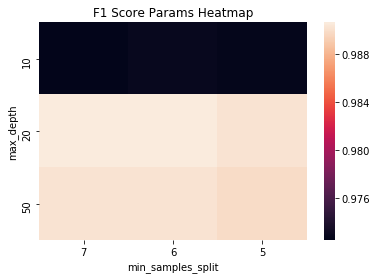
\includegraphics[width=1\linewidth]{f1_heatmap.png}
  \caption{Heatmap around the optimal parameters for the DecisionTreeRegressor.}
  \label{fig:test1}
\end{minipage}%
\hspace{4mm}
\begin{minipage}{.45\textwidth}
  \centering
  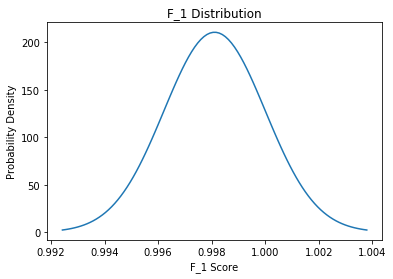
\includegraphics[width=1\linewidth]{f1_dist.png}
  \caption{\scriptsize{Distribution of the $F_1$ score for the best set of parameters.}}
  \label{fig:test2}
\end{minipage}
\end{figure}


\subsection{$\mathit{MRAE_c}$ Score}
The 5-fold \textit{GridSearchCV} using the custom scorer $\mathit{MRAE_c}$ as scoring parameter showed that the best set of parameters for the \textit{DecisionTreeRegressor} are are \textbf{max\_depth: 30} and \textbf{min\_samples\_split: 4}. Subsequently, the $\mathit{MRAE_c}$ score for such set of parameters is $\mathbf{\mathit{MRAE_c}=0.018023652156838658}$ with standard deviation $\mathbf{\sigma_{\mathit{MRAE_c}}=0.00115203}$. The following are visual representations of the previous results.

\begin{figure}[H]
\centering
\begin{minipage}{.45\textwidth}
  \centering
  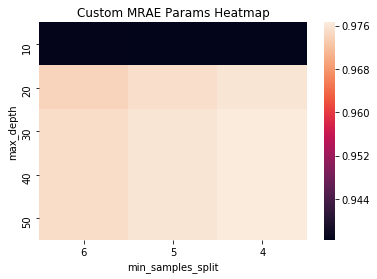
\includegraphics[width=1\linewidth]{mrae_c_heatmap.png}
  \caption{Heatmap around the optimal parameters for the DecisionTreeClassifier.}
  \label{fig:test1}
\end{minipage}%
\hspace{4mm}
\begin{minipage}{.45\textwidth}
  \centering
  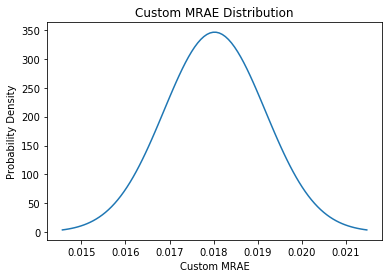
\includegraphics[width=1\linewidth]{mrae_c_dist.png}
  \caption{\scriptsize{Distribution of the $\mathit{MRAE_c}$ score for the best set of parameters.}}
  \label{fig:test2}
\end{minipage}
\end{figure}

\subsection{Final Score}
The final score obtained with this particular design is: $F_s = 1.9800836033636662$. The practical routine of $sklearn$ for the decision tree include a $random\_state$ internal variable. This was set randomly to 42 in order to get reproducible results.


\end{document}